  \begin{subfigure}[b]{0.7\textwidth}
    \centering
    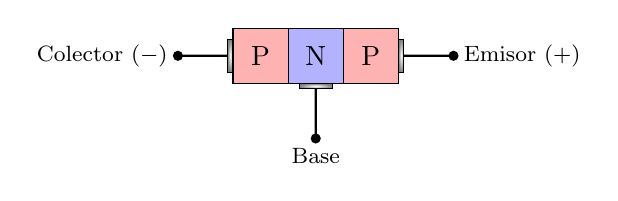
\begin{tikzpicture}[scale=0.7]
      \draw[fill=red!30] (0,0) rectangle node{P} (1,1);
      \draw[fill=blue!30] (1,0) rectangle node{N} (2,1);
      \draw[fill=red!30] (2,0) rectangle node{P} (3,1);
      \filldraw[thick] (-0.1,0.5) -- (-1,0.5) circle (2pt) node[left, font=\footnotesize] {Colector $(-)$};
      \filldraw[thick] (3.1,0.5) -- (4,0.5) circle (2pt) node[right, font=\footnotesize] {Emisor $(+)$};
      \filldraw[thick] (1.5,-0.1) -- (1.5,-1) circle (2pt) node[below, font=\footnotesize] {Base};
      \shadedraw[color=black,fill=gray,inner color=white,outer color=gray] (-0.1,0.2) rectangle (0,0.8);
      \shadedraw[color=black,fill=gray,inner color=white,outer color=gray] (3,0.2) rectangle (3.1,0.8);
      \shadedraw[color=black,fill=gray,inner color=white,outer color=gray] (1.2,-0.1) rectangle (1.8,0);
    \end{tikzpicture}
    \caption{Transistor PNP.}
  \end{subfigure}

  \vspace{5mm}

  \begin{subfigure}[b]{0.7\textwidth}
    \centering
    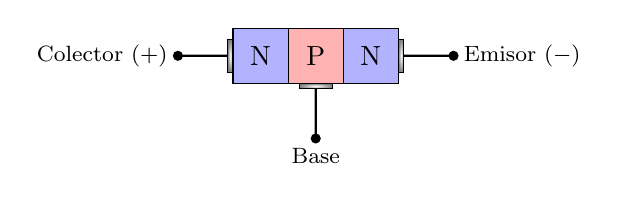
\begin{tikzpicture}[scale=0.7]
      \draw[fill=blue!30] (0,0) rectangle node{N} (1,1);
      \draw[fill=red!30] (1,0) rectangle node{P} (2,1);
      \draw[fill=blue!30] (2,0) rectangle node{N} (3,1);
      \filldraw[thick] (-0.1,0.5) -- (-1,0.5) circle (2pt) node[left, font=\footnotesize] {Colector $(+)$};
      \filldraw[thick] (3.1,0.5) -- (4,0.5) circle (2pt) node[right, font=\footnotesize] {Emisor $(-)$};
      \filldraw[thick] (1.5,-0.1) -- (1.5,-1) circle (2pt) node[below, font=\footnotesize] {Base};
      \shadedraw[color=black,fill=gray,inner color=white,outer color=gray] (-0.1,0.2) rectangle (0,0.8);
      \shadedraw[color=black,fill=gray,inner color=white,outer color=gray] (3,0.2) rectangle (3.1,0.8);
      \shadedraw[color=black,fill=gray,inner color=white,outer color=gray] (1.2,-0.1) rectangle (1.8,0);
    \end{tikzpicture}
    \caption{Transistor NPN.}
  \end{subfigure}
  \caption{Esquema ilustrativo de transistores BJT.}
  \label{fig_ilustracion_bjt}
